\documentclass[11pt]{article}

\usepackage{sectsty}
\usepackage{graphicx}
\usepackage[T1]{fontenc}
\usepackage{multicol}
\usepackage{hyperref}
\usepackage{float}
% Margins
\topmargin=-0.5in
\evensidemargin=0in
\oddsidemargin=0in
\textwidth=6.5in
\textheight=9.0in
\headsep=0.25in

\title{ Analiza modelów regresji do przewidywania liczby ludności w Polsce}
\author{ Krzysztof Kulka
        \\ 272667@student.pwr.edu.pl \\ MSiD Lab Wtorek 9.15 NP }
\date{\today}

\renewcommand{\contentsname}{Spis treści}

\begin{document}
\maketitle	
\pagebreak

% Optional TOC
\tableofcontents
 \pagebreak

%--Paper--

\section{Wstęp}
Problemem projektu jest analiza możliwości modelów regresji liniowej do przewidywania liczby ludności w Polsce. W tym celu wykorzystane zostaną dane historyczne dotyczące demografi, oraz innych czynników wpływających na liczebność populacji.
Przedstawiona analiza ma na celu rozstrzygnięcie czy model regresji liniowej jest odpowiedni do przewidywania liczby ludności w Polsce, oraz jakie modele sprawdzają się do tego najlepiej.
Analizie zostaną poddane następujące czynniki:
\begin{itemize}
\item Historyczna liczba ludności
\item Imigracja do kraju
\item Wskaźnik dzietności
\item Oczekiwana długość życia
\item Urbanizacja
\item Wskaźnik zmiany populacji na przestrzeni ostatnich 5 lat
\end{itemize}
Zbadane zaś zostaną następujące modele regresji:
\begin{itemize}
\item Regresja liniowa
\item Regresja typu Ridge
\item Regresja Lasso
\item Regresja Elastic Net
\item Regresja Bayesian Ridge
\end{itemize}
\section{Zbiór danych i jego analiza}
\subsection*{Opis zbioru danych}
Zbiór danych zawiera informacje na temat historycznej liczby ludności, imigracji do kraju, wskazniku dzietnosci, oczekiwanej długości życia w momencie urodzenia na przestrzeni lat 1960-2023.
Dane zostały pobrane z serwisu internetowego World Bank\cite{wbd} Dane dotyczą około 260 krajów. 
Dodatkowo informacje na temat urbanizacji
zostały pobrane z serwisu internetowego Zintegrowana Platforma Edukacyjna Ministerstwa Edukacji Narodowej\cite{zpe}, a wskaźnik zmiany populacji na przestrzeni ostatnich 5 lat został obliczony na podstawie danych historycznych.
\subsection*{Analiza danych}
Do analizy eksploracyjnej danych wykorzystano bibliotekę pandas-profiling\cite{pp}
\subsection*{Populacja w Polsce}
\begin{figure}[H]
        \centering
        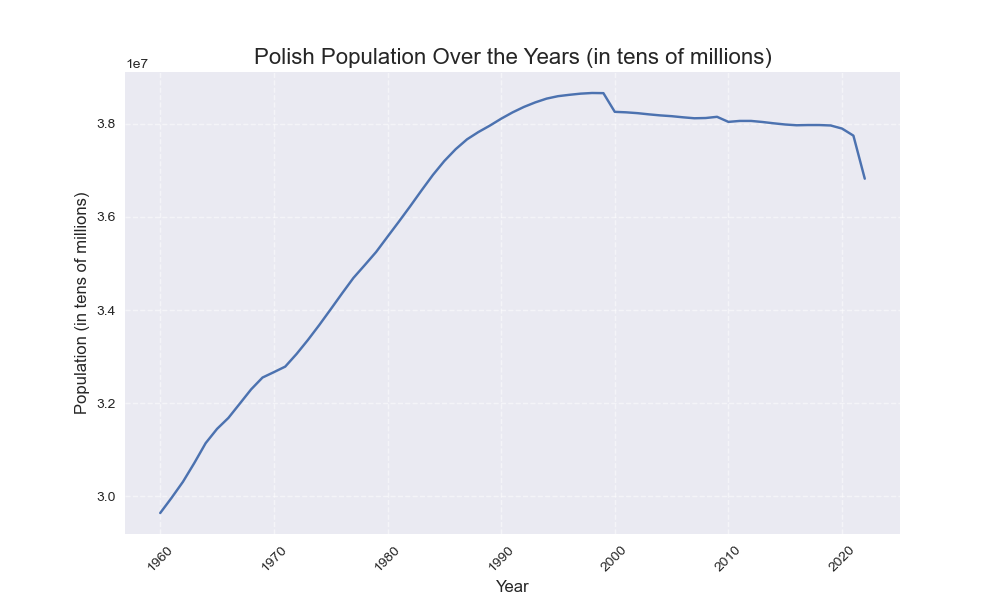
\includegraphics[width=0.8\textwidth]{polish_population_over_the_years.png}
        \caption{Wizualizacja liczby ludności w Polsce na przestrzeni lat}
\end{figure}
\begin{figure}[H]
        \centering
        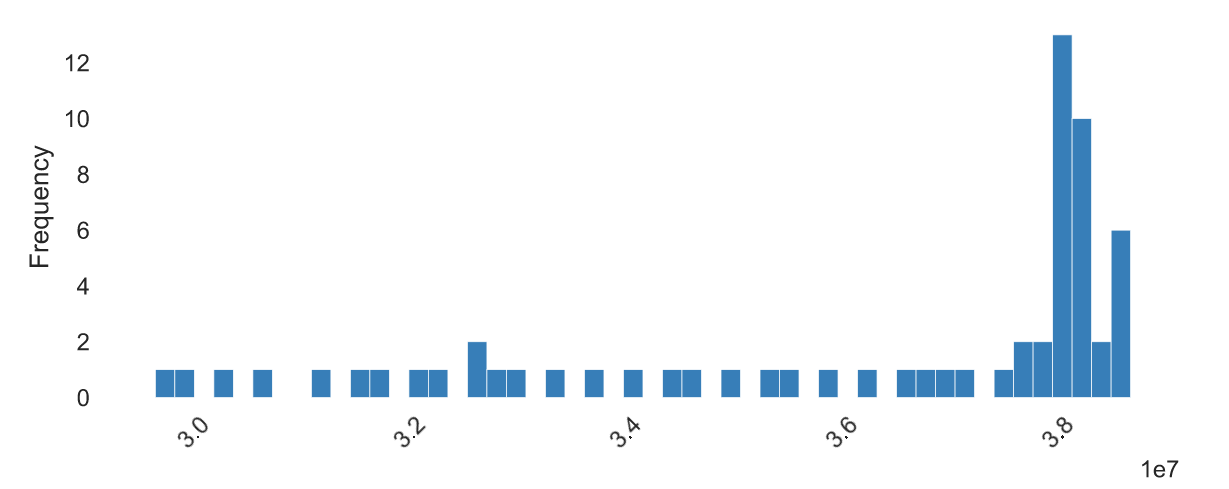
\includegraphics[width=0.8\textwidth]{images/histogram_populacja.png}
        \caption{Histogram liczby ludności w Polsce}
\end{figure}
\begin{table}[H]
        \centering
        \begin{tabular}{|l|l|l|}
        \hline
        Minimum & Maximum & Mediana \\ \hline
        29637450 & 38663481 & 37899070 \\ \hline
        \end{tabular}
        \caption{Statystyki liczby ludności w Polsce}
        \end{table}
\subsection*{Imigracja do Polski}
\begin{figure}[H]
        \centering
        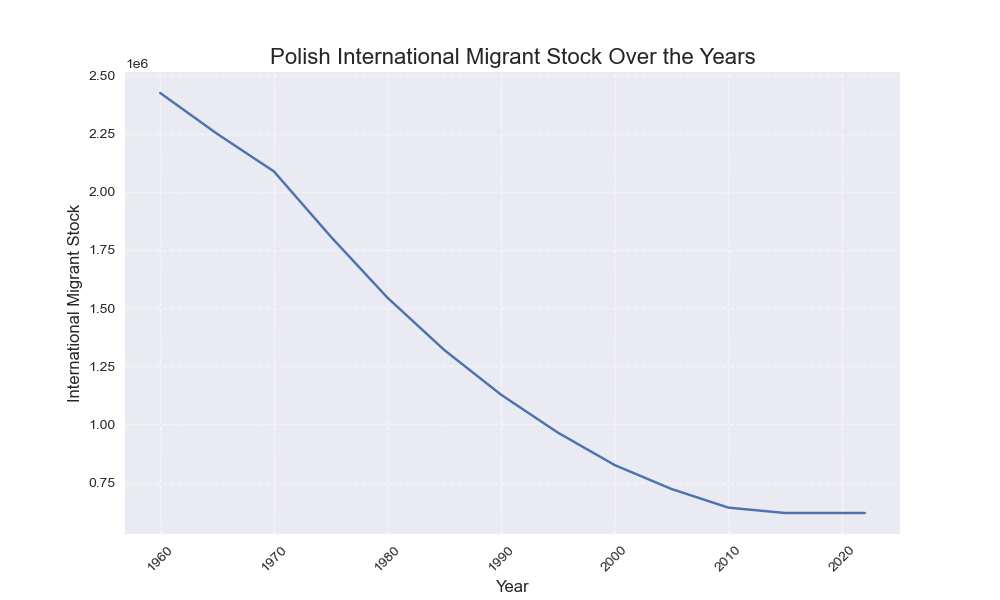
\includegraphics[width=0.8\textwidth]{polish_int_migrant_stock_over_the_years.png}
        \caption{Wizualizacja imigracji do Polski na przestrzeni lat}
\end{figure}
\begin{figure}[H]
        \centering
        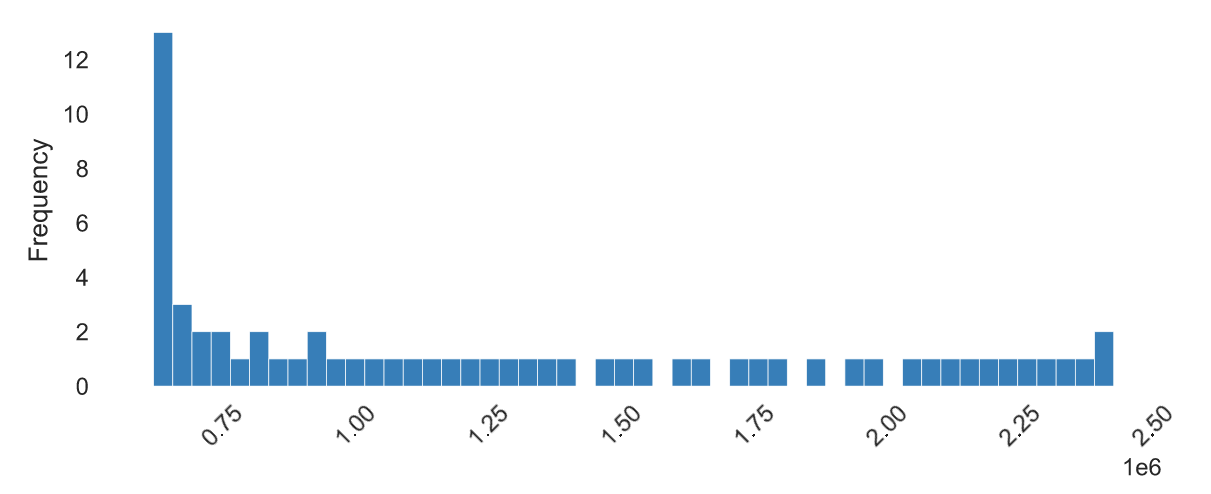
\includegraphics[width=0.8\textwidth]{images/histogram_imigracja.png}
        \caption{Histogram imigracji do Polski na przestrzeni lat}
\end{figure}
\begin{table}[H]
        \centering
        \begin{tabular}{|l|l|l|}
        \hline
        Minimum & Maximum & Mediana \\ \hline
        0 & 0 & 0 \\ \hline
        \end{tabular}
        \caption{Statystyki imigracji do Polski}
        \end{table}
\subsection*{Współczynnik dzietności}
\begin{figure}[H]
        \centering
        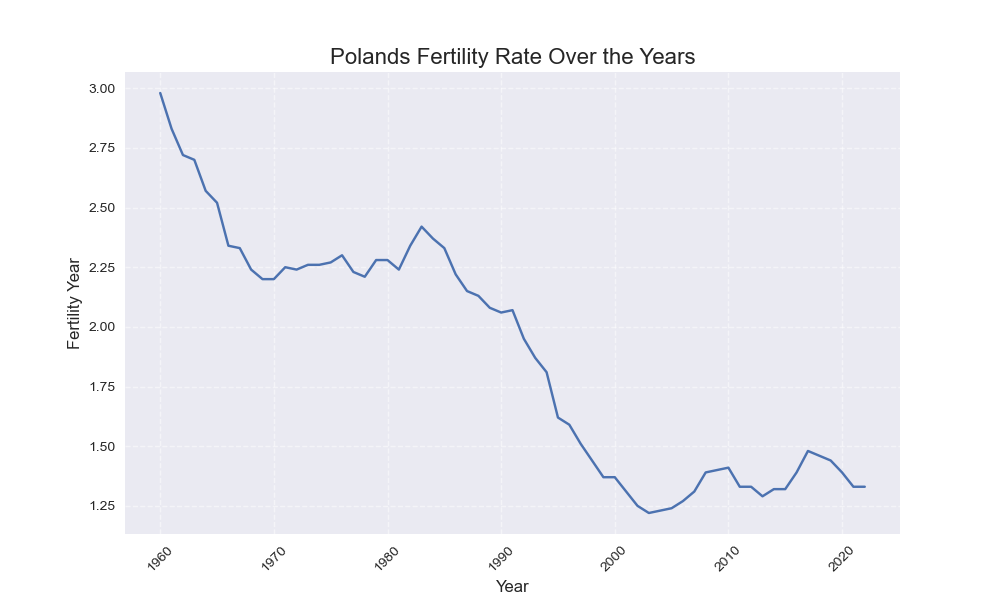
\includegraphics[width=0.8\textwidth]{polish_fertility_rate.png}
        \caption{Wizualizacja współczynnika dzietności Polski na przestrzeni lat}
\end{figure}
\begin{figure}[H]
        \centering
        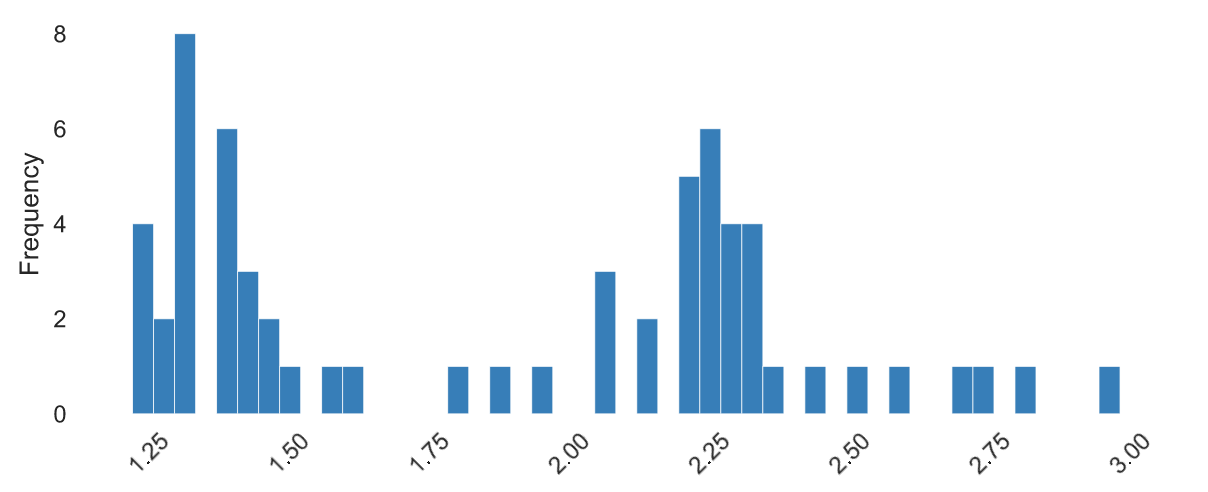
\includegraphics[width=0.8\textwidth]{images/histogram_dzietnosc.png}
        \caption{Histogram współczynnika dzietności na przestrzeni lat}
\end{figure}
\begin{table}[H]
        \centering
        \begin{tabular}{|l|l|l|}
        \hline
        Minimum & Maximum & Mediana \\ \hline
        1.4 & 1.6 & 1.5 \\ \hline
        \end{tabular}
        \caption{Statystyki współczynnika dzietności}
        \end{table}
\subsection*{Oczekiwana długość życia}
\begin{figure}[H]
        \centering
        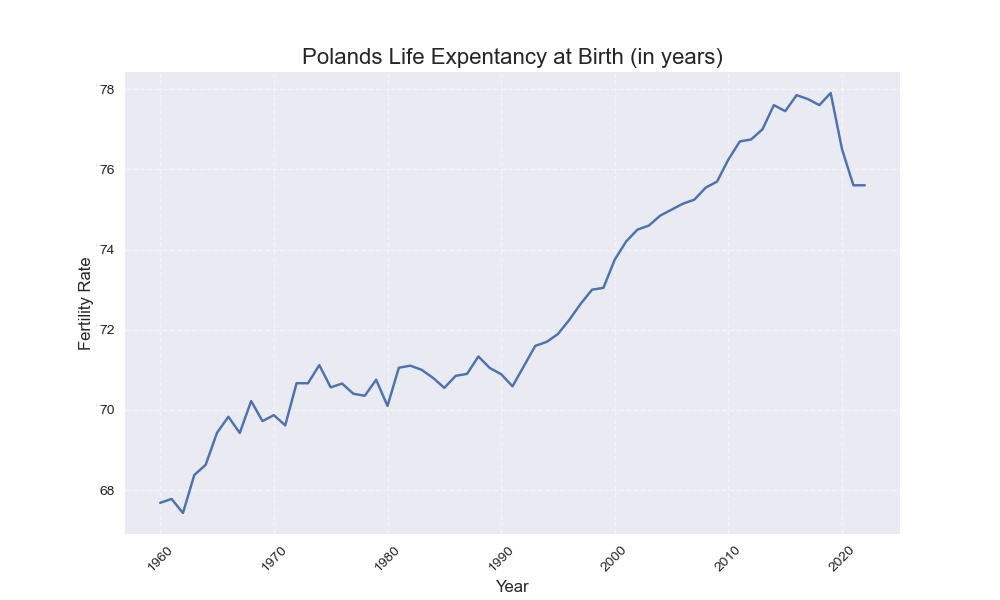
\includegraphics[width=0.8\textwidth]{polish_life_expentancy.png}
        \caption{Wizualizacja oczekiwanej długości życia na przestrzeni lat}
\end{figure}
\begin{figure}[H]
        \centering
        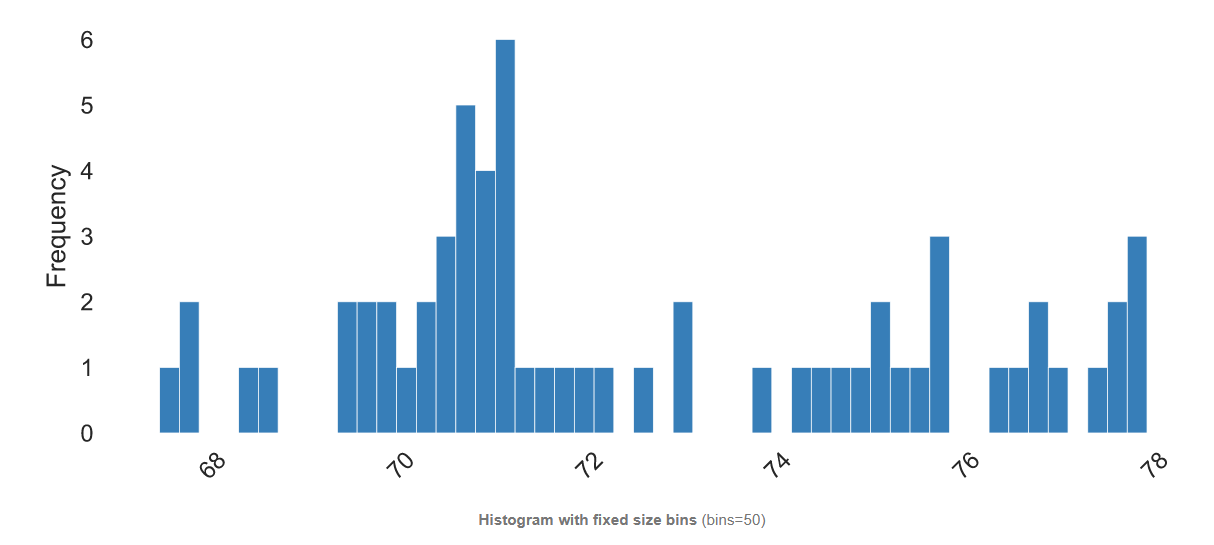
\includegraphics[width=0.8\textwidth]{images/histogram_dl_zycia.png}
        \caption{Histogram oczekiwanej długości życia na przestrzeni lat}
\end{figure}
\begin{table}[H]
        \centering
        \begin{tabular}{|l|l|l|}
        \hline
        Minimum & Maximum & Mediana \\ \hline
        70.0 & 80.0 & 75.0 \\ \hline
        \end{tabular}
        \caption{Statystyki oczekiwanej długości życia}
        \end{table}
\subsection*{Urbanizacja}
\begin{figure}[H]
        \centering
        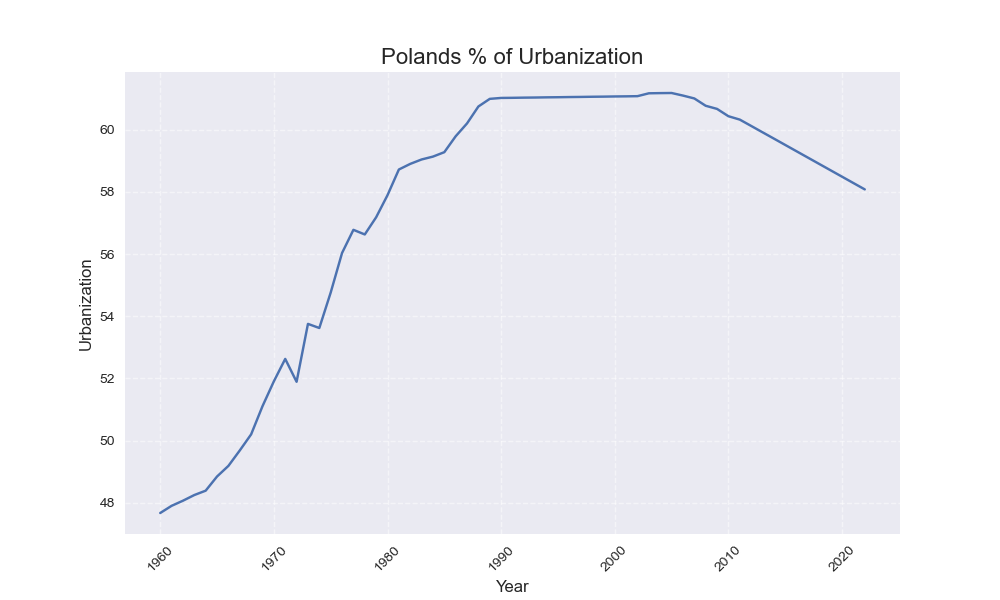
\includegraphics[width=0.8\textwidth]{polish_urbanization.png}
        \caption{Wizualizacja urbanizacji na przestrzeni lat}
\end{figure}
\begin{figure}[H]
        \centering
        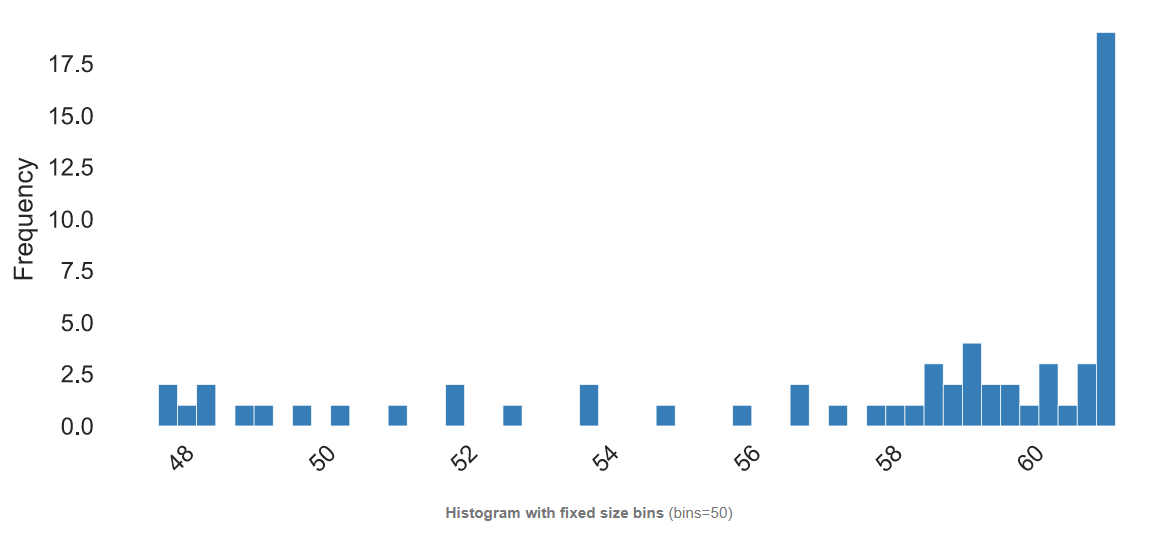
\includegraphics[width=0.8\textwidth]{images/histogram_urbanizacja.png}
        \caption{Wizualizacja urbanizacji na przestrzeni lat}
\end{figure}
\begin{table}[H]
        \centering
        \begin{tabular}{|l|l|l|}
        \hline
        Minimum & Maximum & Mediana \\ \hline
        0.0 & 0.0 & 0.0 \\ \hline
        \end{tabular}
        \caption{Statystyki urbanizacji}
        \end{table}
\subsection*{Wskaźnik zmiany populacji}
\begin{figure}[H]
        \centering
        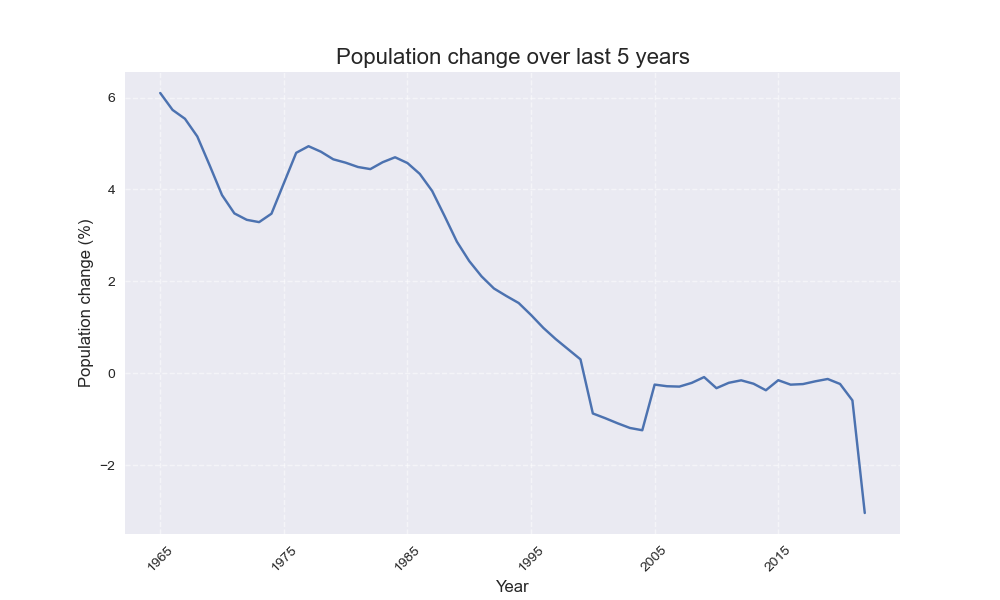
\includegraphics[width=0.8\textwidth]{polish_pop_change_5_years.png}
        \caption{Wizualizacja wskaźnika zmiany populacji na przestrzeni lat}
\end{figure}
\begin{figure}[H]
        \centering
        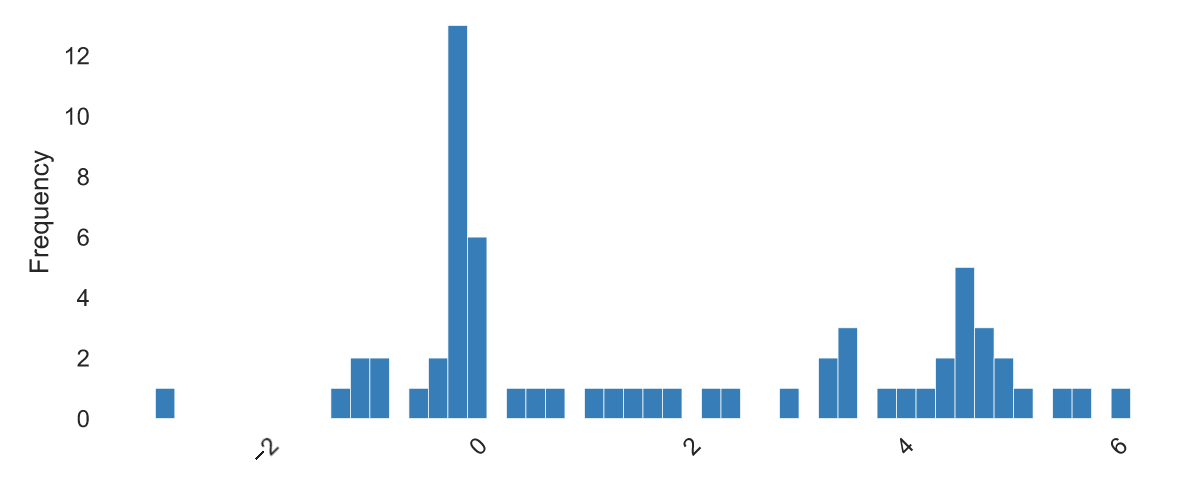
\includegraphics[width=0.8\textwidth]{images/histogram_zmiana_populacji.png}
        \caption{Histogram zmiany polskiej populacji na przestrzeni ostatnich 5 lat}
\end{figure}
\begin{table}[H]
        \centering
        \begin{tabular}{|l|l|l|}
        \hline
        Minimum & Maximum & Mediana \\ \hline
        -0.0001 & 0.0001 & 0.0 \\ \hline
        \end{tabular}
        \caption{Statystyki wskaźnika zmiany populacji}
        \end{table}
\subsection*{Korelacja}
\begin{figure}[H]
        \centering
        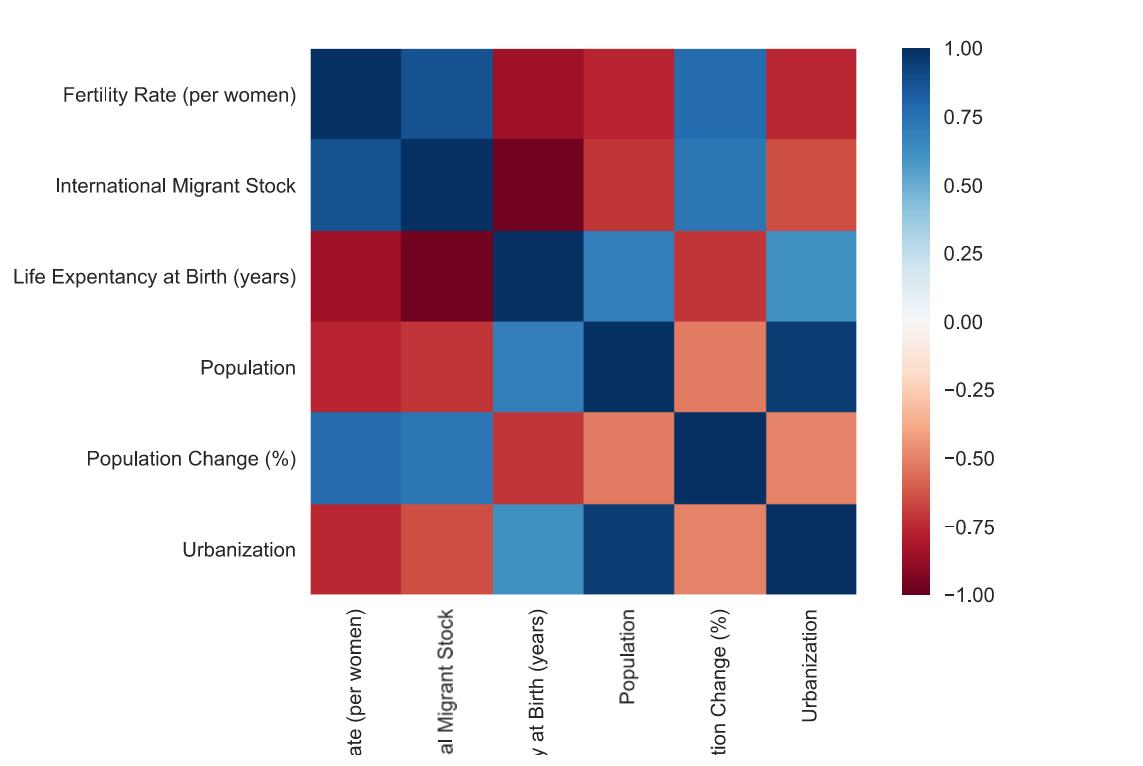
\includegraphics[width=0.8\textwidth]{images/matryca_korelacji.png}
        \caption{Macierz korelacji}
\end{figure}
        Z racji ręcznego dobioru danych i ich selekcji, analiza wykazała bardzo dużą korelację (oraz antykorelacje) pomiędzy wybranymi współczynnikami.
        Pojawia się bardzo zaskakująca, przecząca logice korelacja, pomiędzy współczynnikiem dzietności a populacją wynosząca -0.763.
        Prawdopodobnie wynika ona z tego że przez większość badanego okresu, współczynnik był nadal na bardzo wysokim poziomie, więc mimo że malał, to populacja stale się zwiększała.
        Analogicznie zaskakuje negatywna korelacja migracji z populacją, co jest zaskakujące, ponieważ zgodnie z intuicją, imigracja powinna zwiększać populację.
        Prawdopodobnie wynika to z faktu, że dane dotyczące imigracji są niewielkie, co powoduje że słabo, choć wciąż, przekładają się na polską populację.
        Jeśli zaś chodzi o spodziewane korelacje, należy szczególnie zwrócić uwagę:
        \begin{itemize}
        \item Oczekiwana długość życia z populacją: 0.683
        \item Urbanizacja z populacją: 0.949
        \item Urbanizacja z oczekiwaną długością życia: 0.611
        \end{itemize}
        Korelacje te dobrze wróżą dla modeli regresji, ponieważ są one na tyle silne, że powinny pozwolić na skuteczne przewidywanie liczby ludności w Polsce.
\subsection*{Obróbka danych}
\subsubsection*{Pozyskanie danych}
Najważniejszym krokiem w obróbce danych było wyizolowanie danych dotyczących Polski, oraz usunięcie kolumn, które nie były istotne dla analizy.
Dodatkowo, z racji tego że dane dotyczące imigracji rejestrowane co pięć lat, skorzystano z interpolacji liniowej, aby uzupełnić brakujące dane.
Największe wyzwanie pojawiło się z danymi dotyczącymi urbanizacji. Jedyne z zaufanego oficjalnego źródła były w formie obrazka .jpg.
Aby więc uzyskać dane, i móc zamienić je w data frame, użyto następujących kroków:
\begin{itemize}
\item Scraping obrazka za pomocą skryptu pythonowego
\item Następnie przekazanie zescrapowanego obrazka do zewnętrznego programu WebPlotDigitizer\cite{wpd}
\item Dalej, z racji niedoskonałości otrzymanego wyniku (m.in. potraktowanie lat jako liczb rzeczywistych, a nie całkowitych), dane zostały poprawione za pomocą kolejnego skryptu napisanego w pythonie.
\item Finalnie, ponieważ dane sięgały jedynie 2012 roku, dodano za pomocą skryptu dane z lat 2013-2022 korzystając ze witryny Gegrafia24.pl\cite{gf24}. 
\end{itemize}
\begin{figure}[H]
        \centering
        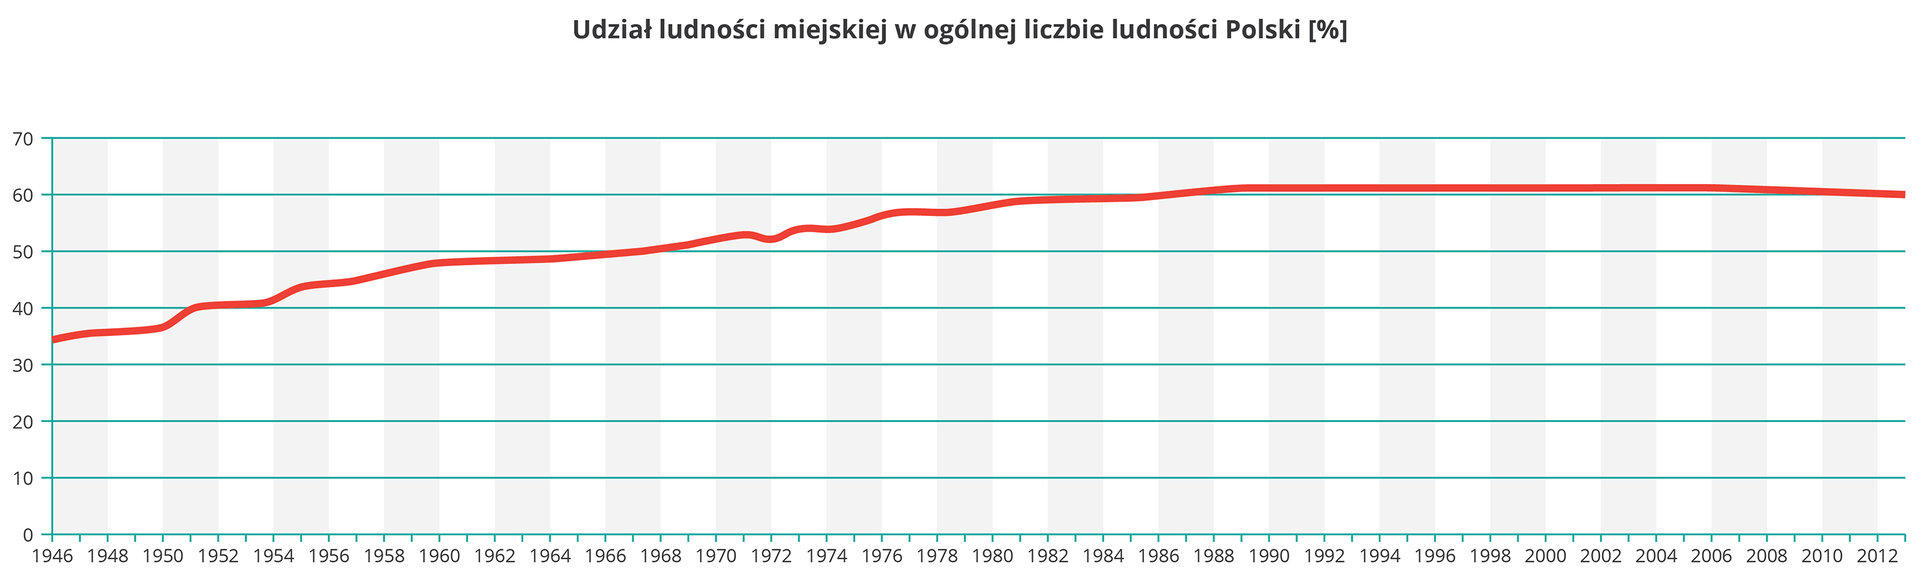
\includegraphics[width=0.8\textwidth]{urbanizacjawPolsce.png}
        \caption{Zescrapowany graf urbanizacji w Polsce}
\end{figure}
\subsubsection*{Eliminacja danych odstających}
Podczas przeglądania grafów reprezentujących zebrane dane, nie trudno było zauważyć że dane po 2019 roku są znacznie odstające od reszty.
Oczywistym jest że w 2020 roku, z racji pandemii, wiele wskaźników uległo zmianie, co sprawia że dane z tego roku są nieprzydatne do analizy.
Z tego powodu, dane z 2020 roku wzwyż zostały usunięte.
\section{Dobór metryk oceny}
Zanim przystąpimy do analizy modeli, należy zdefiniować metryki, które pozwolą nam ocenić ich skuteczność.
Dobór odpowiednich metryk jest kluczowy, ponieważ pozwala na obiektywną ocenę modeli, oraz porównanie ich ze sobą.
W przypadku regresji, najczęściej stosowanymi metrykami są:
\begin{itemize}
\item Mean Squared Error (MSE) - średni błąd kwadratowy
\item Mean Absolute Percentage Error (MAPE) - średni błąd procentowy bezwzględny
\item R2 Score - współczynnik determinacji
\end{itemize}
\subsection*{Mean Squared Error}
MSE jest jedną z najczęściej stosowanych metryk w regresji. Oblicza ona średni błąd kwadratowy pomiędzy wartościami przewidywanymi przez model, a wartościami rzeczywistymi.
\begin{equation}
MSE = \frac{1}{n} \sum_{i=1}^{n} (y_i - \hat{y_i})^2
\end{equation}
\subsection*{Mean Absolute Percentage Error}
MAPE jest metryką, która mierzy średni błąd procentowy bezwzględny pomiędzy wartościami przewidywanymi przez model, a wartościami rzeczywistymi.
\begin{equation}
MAPE = \frac{1}{n} \sum_{i=1}^{n} \frac{|y_i - \hat{y_i}|}{y_i}
\end{equation}
\subsection*{R2 Score}
R2 Score jest metryką, która mierzy jak dobrze model przewiduje dane w porównaniu do średniej wartości. Wartość R2 Score może przyjmować wartości od $-\infty$
  do 1, gdzie 1 oznacza idealne dopasowanie modelu.
\begin{equation}
R2 = 1 - \frac{\sum_{i=1}^{n} (y_i - \hat{y_i})^2}{\sum_{i=1}^{n} (y_i - \bar{y})^2}
\end{equation}
\section{Analiza modeli}
\subsection*{Dla podziału 80/20}
Podział 80/20 oznacza to że model uczyć będzie się na danych z lat 1960-2008, a testowany będzie na danych z lat 2009-2019.
\subsubsection*{Regresja liniowa}
\begin{figure}[H]
        \centering
        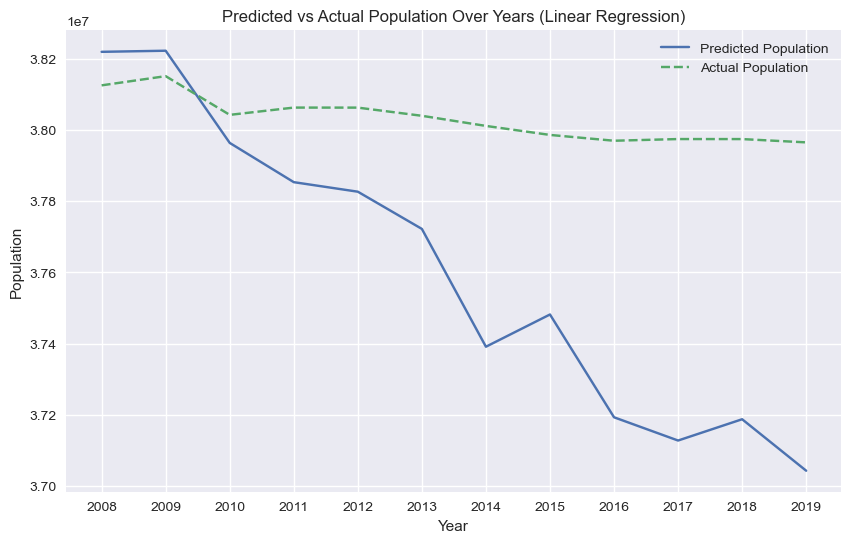
\includegraphics[width=0.8\textwidth]{images/linear.png}
        \caption{Regresja liniowa}
\end{figure}
\subsubsection*{Regresja Ridge}
\begin{figure}[H]
        \centering
        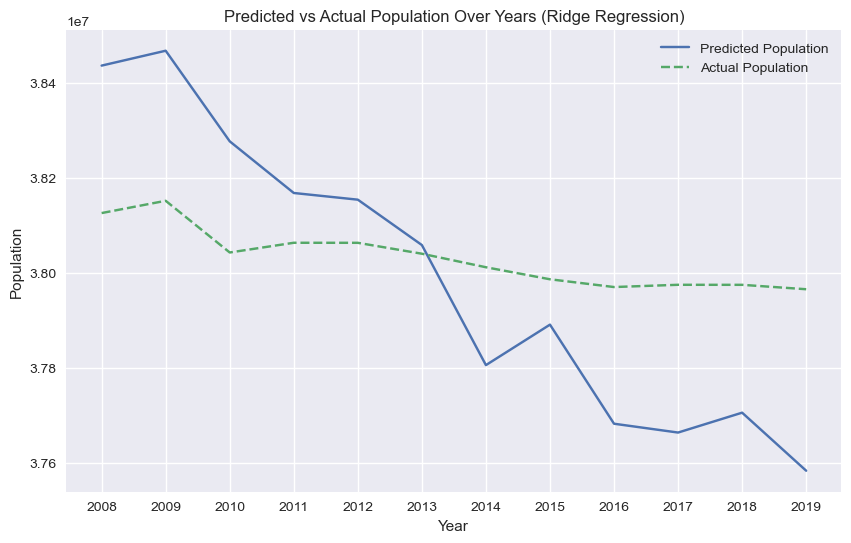
\includegraphics[width=0.8\textwidth]{images/ridge.png}
        \caption{Regresja Ridge}
\end{figure}
\subsubsection*{Regresja Lasso}
\begin{figure}[H]
        \centering
        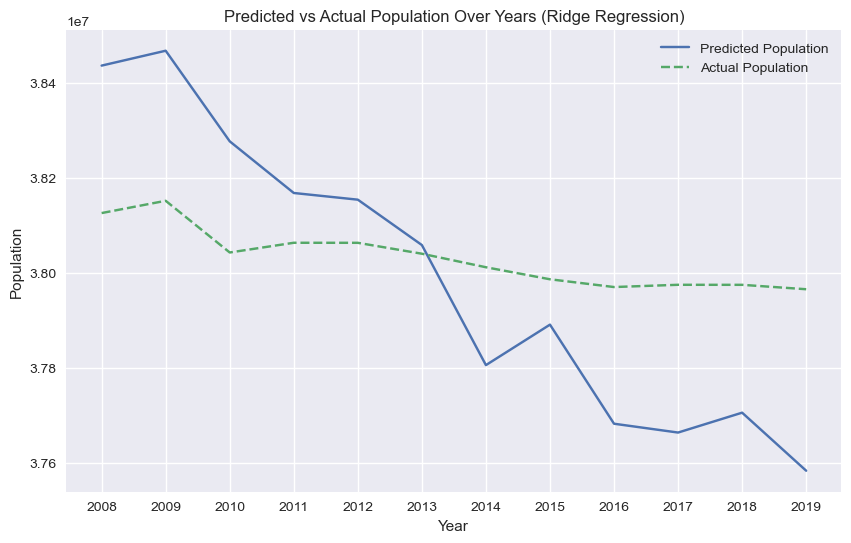
\includegraphics[width=0.8\textwidth]{images/lasso.png}
        \caption{Regresja Lasso}
\end{figure}
\subsubsection*{Regresja Elastic Net}
\begin{figure}[H]
        \centering
        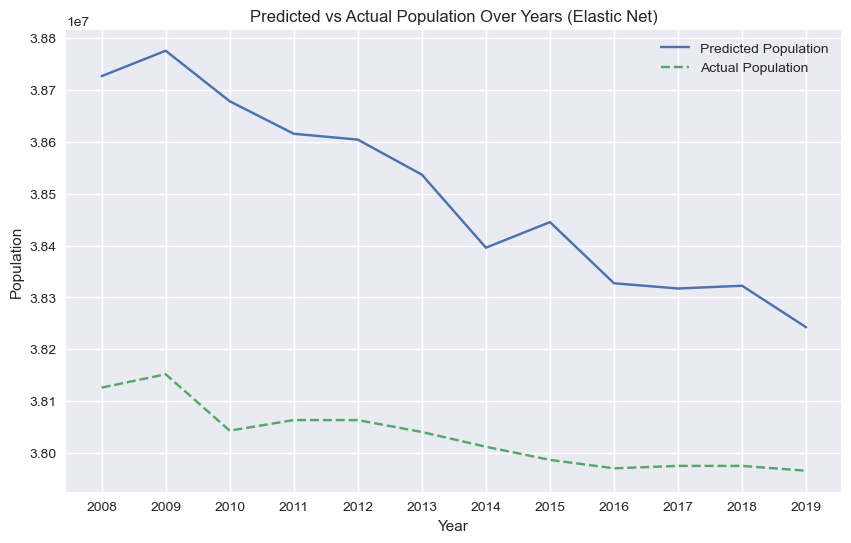
\includegraphics[width=0.8\textwidth]{images/elastic_net.png}
        \caption{Regresja Elastic Net}
\end{figure}
\subsubsection*{Regresja Bayesian Ridge}
\begin{figure}[H]
        \centering
        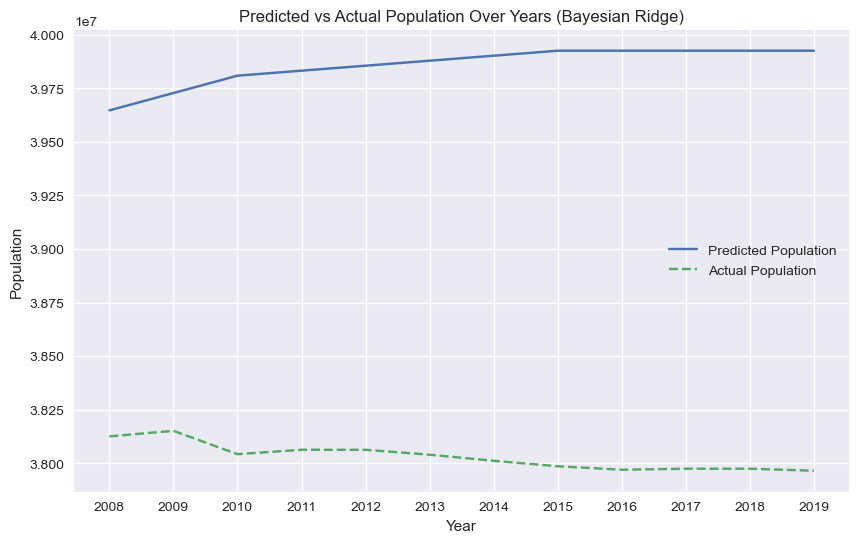
\includegraphics[width=0.8\textwidth]{images/bayesian_ridge.png}
        \caption{Regresja Bayesian Ridge}
\end{figure}
\begin{table}[H]
        \centering
        \begin{tabular}{|l|l|l|l|}
        \hline
        Model & MSE & MAPE & R2 Score \\ \hline
        Linear Regression & 1.07e+13 & 0.03 & 0.99 \\ \hline
        Ridge Regression & 1.07e+13 & 0.03 & 0.99 \\ \hline
        Lasso Regression & 1.07e+13 & 0.03 & 0.99 \\ \hline
        Elastic Net & 1.07e+13 & 0.03 & 0.99 \\ \hline
        Bayesian Ridge & 1.07e+13 & 0.03 & 0.99 \\ \hline
        \end{tabular}
        \caption{Wyniki dla podziału 80/20}
        \end{table}
\bibliographystyle{plain}
\bibliography{bibliografia}
\end{document}
